% COMS 6998, Fall 2026 -- P2 updated from independently accepted P19 evidence.
% New version; original submission-b5 and official IEEE class remain unchanged.
\documentclass[conference,10pt,letterpaper]{IEEEtran}
\usepackage[T1]{fontenc}
\usepackage{cite}
\usepackage{graphicx}
\usepackage{booktabs}
\usepackage{tabularx}
\usepackage{flushend}
\usepackage[hyphens]{url}
\usepackage[hidelinks]{hyperref}

\newcommand{\field}[1]{\textit{[#1]}}

\title{B5: E-Graph-Augmented Tool-in-the-Loop RTL Verification}
\author{\IEEEauthorblockN{Chiyu Chen (cc5583), Mingyuan Zheng (mz3143), Yiwen Chen (yc4653)}
\IEEEauthorblockA{COMS 6998: AI-Native Computing $\mid$ Fall 2026\\
P2: Prototype \& Pilot Results $\mid$ Due November 9, 2026, 11:59 PM ET}}

\begin{document}
\maketitle
\thispagestyle{plain}
\pagestyle{plain}

\section{Project Goal and Updates}
Our project asks whether E-graph semantic feedback helps an LLM verify RTL more
effectively and efficiently than raw execution feedback. The proposal compares
text-only (A), raw-coverage (B), and E-graph-enhanced (C) stimulus generation.
Exploratory coverage pilots implement that original track. The separately
authorized \emph{test2} extension fixes stimuli and generates passive
SystemVerilog monitors, measuring valid fault detection, false alarms, and cost.
This separates a generated checker's quality from the model's input-selection
ability while testing the same semantic-feedback hypothesis.

The endpoint change is explicit: changing a monitor under fixed stimuli does
not improve DUT coverage. Raw RTL counters provide workload context; monitor
quality is the outcome. We do not claim an official CVDP or Pass@1 evaluation.
For P2, we now have a completed, independently audited controller retest of the
implemented pipeline. It reuses a published benchmark, so it is not a new hidden
test or cross-IP generalization result. The current scope ends at this milestone;
cross-IP execution remains paused.

\section{Method Overview}
We freeze the DUT, specification, input traces, independent reference, model
settings, selection rule, and resource limits before comparing B and C. Python
orchestrates candidate generation, compilation, public development feedback,
per-round snapshots, release, and common grading. A Rust \texttt{egg} pipeline
forms restricted equivalence groups; independent Z3 checks preserve widths,
signedness, complete activation guards, and clock/reset context. These establish
limited two-state combinational relations, not general sequential or four-state
equivalence. Equivalent guards retain their original source counters.

A Claude-authored specification checker remains independent of GPT candidate
monitors; candidates never grade themselves. B receives the permitted
specification/RTL, fixed development observations, raw counters, and its own
previous candidate/development feedback. C adds validated E-graph relations.
The current prompts exclude reference code, mutant sources, final evaluation
observations, and solver witnesses. Withholding them from these requests does
not make the previously published corpus fresh hidden data.

The new retest uses \texttt{gpt-6.1-sol}/low, one independent session per arm and
three rounds, interleaved B1,C1,C2,B2,B3,C3. Model and registered resource policy
are shared, including an 8,192-output-token ceiling; equal limits do not mean
equal realized tokens. All six candidates freeze before one grading pass, and
each final is its last compile-valid candidate, never selected by final score.
A final-post \texttt{trace\_done} marker exposes finite trace termination without
adding a DUT input or clock edge.

Correct-DUT controls gate fault credit. A credited alarm must align with an
independent observable violation; an earlier alarm cannot earn credit. Unknowns,
invalid candidates, unobservable faults, and failures remain in the evidence.
Repeated alarms and two simulators do not create extra defect types. Tokens,
candidate compilation, DUT simulation, monitor replay, and wall time are distinct
measurements. Without a token-matched placebo, B/C tests the whole feedback
package, not pure semantic content.

\section{Prototype and Pilot Results}
\textbf{Current end-to-end prototype.} The multi-cycle request/response controller
uses frozen inputs under \path{test2/tasks/axis_length_done_v1/}. The new
registration is \path{test2/configs/controller_done_bc_retest_v3.json}; the entry
is \path{test2/retest_v3/cli.py}. The saved run in
\path{test2/results/controller-done-bc-retest-v3/} binds prompts, responses,
\texttt{release.json}, final selections, usage, and scores. It completed once:
six generations, compilation/development feedback, all-round freeze, then common
grading and report. There were no retries or remote token-count calls. P19
independently checked saved evidence; it did not generate another cohort.

Earlier infrastructure failures remain archived. The historical pilot's
catalog-field audit failure required read-only recovery; a later adapter
qualification rejected missing returned service tiers. Those versions and
counterexamples are preserved. The accepted R03 adapter repaired that gate
before the current live retest; no old outcome was relabeled.

\begin{figure*}[t]
\centering
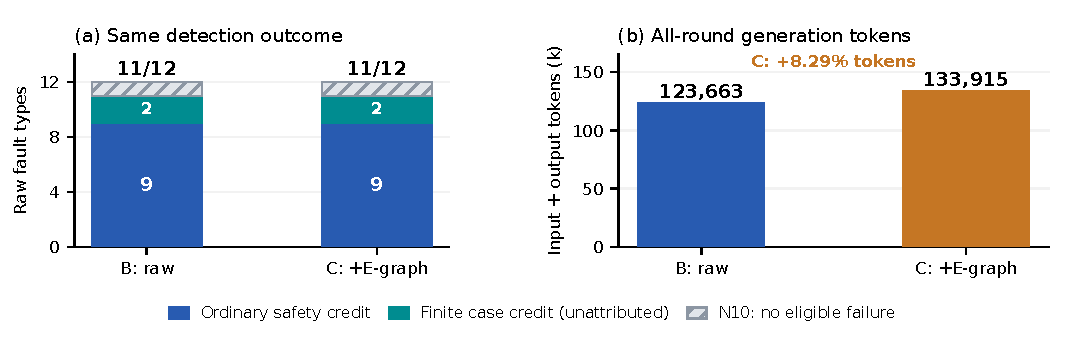
\includegraphics[width=\textwidth]{images/retest-bc.pdf}
\caption{P19-audited controller retest: one independent session per arm, three
rounds each (six generation calls), on the same published fixed-stimulus corpus.
Left: both final monitors have the same raw union of 11/12 fault types: nine
ordinary-safety types plus two end-marker finite case types, \emph{unattributed}
to a specific monitor property. Gray N10 has no eligible reference failure and
remains in the raw denominator. Right: actual generation input+output totals
over all three rounds, B 123,663 and C 133,915 (+8.2903\%). No averaging or
independent-repeat error bars are implied. Cache/reasoning tokens are subsets,
not added again; this is not an invoice or a correctness proof.}
\label{fig:retest}
\end{figure*}

\textbf{Latest comparison.} Both arms already reach the same case/type union in
round~1 and retain it in rounds~2--3 (Fig.~\ref{fig:retest}); both finals select
round~3. Each candidate passes 18 finite correct controls. The raw inventory is
12 fault types/144 fault pairs plus 18 controls, or 162 cases per candidate.
All 38 reference-unknown pairs remain per round. N10 is a mutant identifier:
its 12 frozen reference outcomes are PASS, with no eligible fault evidence.
Separately, input completion is 0/10 eligible N01 pairs, all retaining reference
unknown. Neither fact is silently converted into a pass or removed from the
raw denominator. The finite credit is case-level and unattributed; passing
controls does not prove general monitor soundness or 128-cycle completion.

The new run uses B 116,529 input + 7,134 output tokens and C 127,168 + 6,747.
C spends 8.2903\% more total tokens without extra detections. The combined
conservative usage-based cost upper is \$1.569371, not an actual
provider invoice. The run took 177.995\,s including cleanup, with 12 candidate
compiler processes and 990 monitor replays (18 development + 972 grading),
covering 204,444 replayed cycles. These reuse frozen DUT observations: they are
not new physical DUT simulations, generated stimuli, or formal proofs.

\textbf{Historical cohort, kept separate.} The earlier three-sessions-per-arm,
six-round pilot used 36 generation calls. B totaled 740,643 tokens and C 813,649
(+9.8571\%), with the same final union of 11 observable types and raw denominator
12. Its invalid rounds and costs remain; one B final has 40 total unresolved
pairs rather than 38. The earlier 540 formal jobs still have 75 PASS, 104 FAIL,
and 361 TIMEOUT statuses, including 74 unreproduced/unresolved BMC witnesses.
The new retest does not resolve those outcomes. Neither cohort was rerun to
prepare this paper, and the cohorts are not pooled as independent fresh-hidden
evidence.

The editable source includes \path{figure-data.json}, which binds the retest
ledger/grade, historical audit, and P19 review by hash. All figure values derive
from these saved artifacts; no research experiment was rerun for this paper.

\section{Next Steps}
\textbf{Main risk and paper plan.} Saturation leaves little room for C to improve;
one session per arm, one published workload, and longer C context limit causal
and statistical conclusions. This run shows no additional C benefit here, not
that E-graphs are universally unhelpful. G1 now has P17's limited finite-control
acceptance; that is not a proof of these monitors or a reason to repeat generic
qualification for P2.

A possible Milestone~3 plan (Nov~23), subject to separate future authorization,
would preregister a small nonsaturated obligation set and a genuinely disjoint
holdout before seeing C outcomes, then compare matched conditions and a
token-matched placebo. Any new oracle scope must receive independent Claude
review; GPT will not silently repair it. Existing cross-IP task drafts are
preparation, not implemented or tested multi-IP monitor results. No new
experiment or paid call is promised by this P2 delivery.

\textbf{Actual midterm feedback/response pending.} Authentic instructor/TA
technical feedback has not been found in the bounded local review. We cannot
invent a response: the original comment, resulting change, evidence, and limit
must be recorded when available. User priorities and internal P19 audits do not
substitute for classroom feedback. The two-page draft therefore retains this
content gap and has not been submitted to the course platform.

\end{document}
